\section{Immutable Construction and Accuracy}
\subsection{The cost of building a static filter}
\label{sec:static}
A static filter can be small and fast to query because it receives the complete set before construction. That advantage comes with a cost: adding a new member generally requires rebuilding. Table~\ref{tab:static} includes preparation so that this work does not disappear from the comparison.

\begin{table}[!htbp]\centering\small
\caption{Static construction at 67M input operations. Times are mean seconds over three repetitions; rate columns are means of per-repeat rates in millions per second. Build-only rate uses $D$; end-to-end rate uses $N$ and includes preparation. The latter is stream-processing throughput, not an online insert rate.}
\label{tab:static}
\begin{tabular}{@{}llrrrr@{}}
\toprule
\textbf{Input} & \textbf{Filter} & \textbf{Prep (s)} & \textbf{Build (s)} & \textbf{Build (M keys/s)} & \textbf{Total (M ops/s)} \\
\midrule
Uniform & XOR & 0.447 & 16.640 & 4.09 & 3.99 \\
Uniform & Fuse-style & 0.447 & 10.878 & 6.44 & 6.20 \\
Zipfian & XOR & 2.139 & 0.012 & 18.98 & 31.41 \\
Zipfian & Fuse-style & 2.139 & 0.011 & 20.57 & 31.42 \\
\bottomrule
\end{tabular}

\end{table}

\begin{figure}[!htbp]\centering
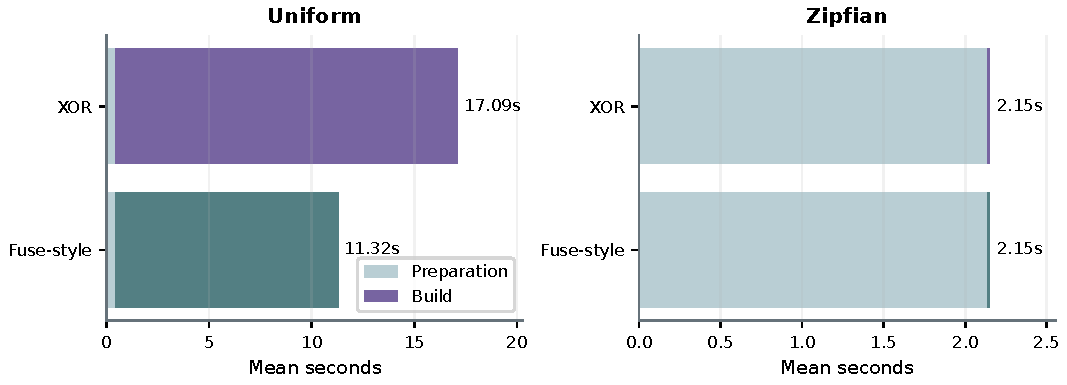
\includegraphics[width=0.96\linewidth]{static_preparation.pdf}
\caption{Mean preparation and build time for the immutable filters. Both are charged the shared preparation step as if built independently from the raw stream. In the actual driver the distinct-key preparation is computed once and reused.}
\label{fig:static-cost}
\end{figure}

For uniform input, preparation is a copy because the audit has verified that the stream is distinct. For skewed input, it sorts and deduplicates all 67M values before the much smaller set is built. Consequently, a high build-only rate on $D$ should not be confused with the end-to-end cost of processing $N$ input operations. Positive lookup rates also benefit from the frequency-weighted query stream, whose hottest keys are revisited often.

XOR uses 9-bit fingerprints at the primary target. The Fuse-style variant uses 10 bits. Its extra bit approximately halves the nominal FPR but also increases storage; it can therefore be larger than XOR here despite the Fuse family's more compact graph layout. We are comparing the actual configured implementations, rather than claiming an equal-accuracy contest between their theoretical storage bounds. Their final packed arrays do not include the substantial graph workspaces required during construction.

\subsection{Why preprocessing changes the construction story}
For skewed input, XOR's build stage takes only about 0.012 seconds, but preparation takes about 2.139 seconds. More than 99\% of the combined time is therefore spent producing the distinct set. The two immutable filters finish in almost the same end-to-end time on this stream even though their build-only rates differ. Under uniform input, the graph build dominates instead: total preparation-plus-build time is about 17.09 seconds for XOR and 11.32 seconds for the Fuse-style variant. The bottleneck changes with the data, not only with the filter family.

\subsection{A lifetime view of an immutable snapshot}
Construction is paid again when a snapshot is rebuilt. If a filter requires preparation time $P$, build time $B$, and then serves $L$ queries at average filter cost $c$, the corresponding filter-only lifetime cost is $P+B+Lc$. This accounting separates a frequently rebuilt snapshot from a long-lived one without treating batch construction as an online insertion rate. Our measurements supply $P$, $B$ and query batch costs; the application must supply its rebuild frequency and query volume. They do not yet supply peak construction memory or the cost of replacing a live snapshot.
\finding{Deduplication makes the stored set small, but the original stream still has to be processed. A static filter should be compared using preparation, construction and the expected lifetime of the snapshot.}
\clearpage

\subsection{Accuracy is a measured rate with uncertainty}
At 67M uniform operations, the half-full primary CQF is expected to have FPR near $0.499\times2^{-9}\approx0.000975$, not exactly the nominal $1/512\approx0.001953$. Under skew, the operation-sized CQF has many fewer distinct fingerprints and a much smaller expected collision rate. Ordinary Bloom and Counting Bloom remain near their nominal target; guarded Blocked Bloom measures about $0.000974$, roughly half that target. These are different achieved operating points.

\begin{figure}[!htbp]\centering
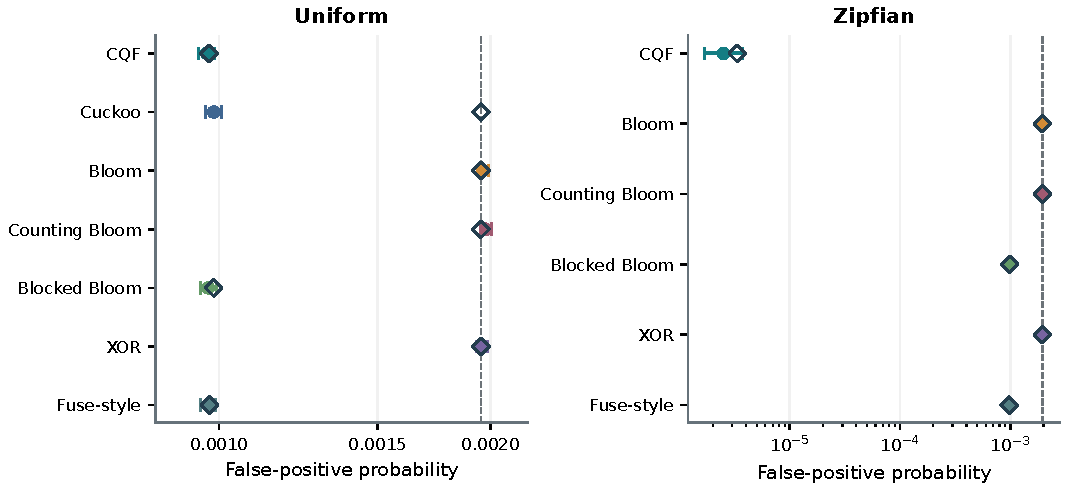
\includegraphics[width=\linewidth]{accuracy_intervals.pdf}
\caption{First-run measured FPR with 95\% Wilson intervals, using 10M negatives for each distribution. Diamonds indicate structure-specific estimates (the full-bucket reference value for Cuckoo); the dashed line marks the common nominal target. Cuckoo's failed skewed case is omitted. Cuckoo has a different random hash realization in each repetition; its repeat range is preserved in the accompanying table.}
\label{fig:accuracy}
\end{figure}

\begin{table}[!htbp]\centering\small
\caption{67M accuracy detail. Intervals use the first repetition and $Q=10$M, without pooling repeated copies of the same queries. The last column gives the range across the three raw timing repetitions. FPRs and interval endpoints are in units of $10^{-3}$.}
\label{tab:accuracy}
\begin{tabular}{@{}llrrr@{}}
\toprule
\textbf{Input} & \textbf{Filter} & \textbf{First FPR} & \textbf{95\% interval} & \textbf{Repeat range} \\
\midrule
Uniform & CQF & 0.9692 & [0.9501, 0.9887] & 0.9692 \\
Uniform & Cuckoo & 0.9865 & [0.9672, 1.0062] & 0.9661--0.9865 \\
Uniform & Bloom & 1.9616 & [1.9344, 1.9892] & 1.9616 \\
Uniform & Counting Bloom & 1.9771 & [1.9498, 2.0048] & 1.9771 \\
Uniform & Blocked Bloom & 0.9730 & [0.9539, 0.9925] & 0.9730 \\
Uniform & XOR & 1.9597 & [1.9325, 1.9873] & 1.9597 \\
Uniform & Fuse-style & 0.9725 & [0.9534, 0.9920] & 0.9725 \\
Skewed & CQF & 0.0025 & [0.0017, 0.0037] & 0.0025 \\
Skewed & Bloom & 1.9577 & [1.9305, 1.9853] & 1.9577 \\
Skewed & Counting Bloom & 1.9276 & [1.9006, 1.9550] & 1.9276 \\
Skewed & Blocked Bloom & 0.9742 & [0.9551, 0.9937] & 0.9742 \\
Skewed & XOR & 1.9322 & [1.9052, 1.9596] & 1.9322 \\
Skewed & Fuse-style & 0.9810 & [0.9618, 1.0006] & 0.9810 \\
\bottomrule
\end{tabular}

\end{table}

For the fixed-hash structures, repeated runs reproduce the same false-positive outcomes. Cuckoo's range also reflects its fresh random hash coefficients. A rate slightly above the nominal target can arise from finite sampling and from the approximation used for sizing; the confidence interval and implementation model provide the relevant context. A wider multi-seed experiment would be needed to establish a robust accuracy guarantee or to compare very small differences between mixers.
\finding{A lower observed FPR can result from spare capacity, a guard bit or fewer distinct members. It should be interpreted together with the memory and sizing policy that produced it.}
\clearpage
